\section{Data}\label{sec:data}
Summarize the DP2 context relevant to calibrations: instrument, filters, observing period/epochs, detector layout, available exposure types (bias/dark/flat/science), and definitions of calibration epochs.
Optionally add science context.

\subsection{LSSTCam and CCD status for DP2}\label{sec:data:lsstcam}

%Describe the filters. (to move to LSSTCam section)

%Describe the sequencer (to do in LSSTCam section)

%Analyzed with updated sequencer (s3v2). (see calibration epoch section)

%\textcolor{red}{to do:} insert map as a percentage of used pixels: dead, bad and the dead ccd are in one color, color for CCDs worst than the median and green for best CCDs.
%Effective area: vignetted masked + defects


\subsection{Calibration System (CalSys)}\label{sec:data:calsys}

LSST uses four calibration systems to construct calibrations. Three of which (the flat-field illuminator, the collimated beam projector, and the Auxiliary telescope) will be used continuously throughout the LSST, while one calibration system (the Camera Calibration Optical Bench) was used to characterize and qualify the LSSTCam CCDs before integration to the Simonyi Survey Telescope at Rubin Observatory.
\textcolor{red}{add citation to Seans SPIE paper.} 
\subsubsection{Camera Calibration Optical Bench}\label{sec:data:calsys:ccob}

To create optical scenes for characterization, the Camera is placed in-line with an optical scene projector called the Camera Calibration Optical Bench (CCOB) \citep{2024SPIE13103E..0WU}.
The CCOB-wide beam is designed to project a uniform monochromatic light source onto the focal plane, thanks to one of six LEDs, each corresponding to a central wavelength in the LSST filter bandpass.
In-lab tests with the CCOB are described in \textcolor{red}{here add citation}, the so-called 'run 7' was the final campaign of testing of LSSTCam at SLAC,
calibrations produced during that run were used as the initial LSSTCam on-sky observations.
%Light is produced by , is controlled by a custom LED driver and fed into an integrating sphere. The light from the integrating sphere is projected onto the focal plane with a minimal ND filter (10\%) attached to a C-mount lens with an adjustable f/stop. The CCOB-wide beam was used in run 6 and run 7.
%\textbf{I mention run 6 and run 7 here - it is not properly introduced. Is it within scope to mention the EO-testing run at the Rubin Observatory L3 CR?}
%One difference between run 6 and run 7 was that the f/stop of the lens was changed from 2.6 to 1.6 (fully open). This was done to try to reduce the effect of the `weather' and the `CMB pattern' two effects that we found in Run 6 at SLAC, and were found to be due to our projection setup (\citet{2024arXiv241113386B}). While changing the f/stop  did reduce the weather pattern, it also caused a much steeper illumination roll-off across the focal plane. We evaluated the weather pattern and illumination roll-off relative to Run 6.
%To reduce the effects of the `weather' and `CMB' but retain uniform illumination across the focal plane, we installed a Lambertian diffuser to the CCOB-wide beam for Run 7. The diffuser used is a $60^o$ diffusing angle unmounted sheet from Edmunds Optics. We found that the diffuser greatly reduced the `weather', eliminated the CMB pattern, more uniformly illuminated the focal plane, with a penalty of decreasing the overall illumination by roughly 35\%. The diffuser was installed for all run 7 record runs using the CCOB Wide Beam.

\textbf{I am not sure how much we want to talk about the CCOB here. If there is a specific focus (qualifying the CCDs before integration), I can revisit this}

\subsubsection{Flat Field Illuminator}\label{sec:data:calsys:flat_field_illuminator}

The Vera C. Rubin Observatory's Flatfield Calibration System is designed to provide a stable, uniform, and well-characterized illumination required to measure the absolute and relative instrumental responses of the LSST Camera. Operating in tandem with the CBP and AuxTel, this system aims to satisfy a photometric precision of 5 millimag in repeatability and 10 mmag in spatial uniformity across the sky. \textbf{Cite a flatfield calib system paper} The physical architecture of the flatfield system is driven by the fast ($f/1.2$) optical configuration of the Simonyi Survey telescope, which demands exceptional control over both the angular and spatial uniformity of the calibration wavefront. The system directs light toward a large 10.27-meter diameter Lambertian calibration screen that is tilted to 23 degrees to align precisely with the optical axis of the telescope. Because the calibration hardware must co-rotate dynamically with the observatory dome during operations, the primary illumination sources, environmental enclosures, and projection optics are mounted directly onto the dome structures rather than a static mount.

To deliver both broadband and monochromatic illumination during the LSST, the system integrates two independent illumination subsystems within a single centralized optical projector, positioned at the geometric center of the calibration screen structure. Broadband "whitelight" illumination is provided by a specialized module featuring a collection of 10 high-power LEDs selected to span the complete $ugrizy$ filter passbands, with one LED within the $u$ passband with the other five passbands each getting coverage from two LEDs. For monochromatic calibration, the system incorporates a tunable laser system that provides continuous wavelength coverage from 300 to 2600 nm at a 1 kHz pulse rate. This laser can deliver narrow tuning steps between 0.05 and 1 nm and a spectral linewidth under 1 nm FWHM.\textbf{Cite a paper by Parker on this} 
%The hardware is housed in a dedicated 590 kg environmentally controlled enclosure on the dome platform to minimize transmission losses across its 20-meter optical fiber runs. Both illumination sources feed into the projector optics to emit an $\sim f/4$ beam at a working distance of 3.2 meters, filling a 74.1 cm diameter monolithic aluminum aspheric reflector mounted via an adjustable hexapod at the top end of the telescope to cast a flat pupil image onto the screen. The output beam's intensity and spectral content are continuously tracked by an in-dome monitoring suite consisting of a NIST-calibrated silicon photodiode read out by an electrometer alongside two fiber-fed spectrographs covering a combined range of 315-1150 nm.

The data products generated by these dual operating modes support separate but complementary calibration goals within the Rubin DM pipeline, to ensure uniformity across the LSSTCam focal plane. In the DP2 dataset, the flatfields used during ISR are constructed with a weighted combination of the two LEDs within the passband (or the single LED in the case of $u$ band). These data products enable the correction of detector-level systematics, including gain variations, charge transfer inefficiencies, pixel-level defects, and sensor distortions induced by the brighter-fatter effect. The monochromatic flatfield data products from the tunable laser are not used in DP2, but will be utilized in future data releases to map the system's chromatic throughput as a function of focal plane position.

\subsubsection{Collimated Beam Projector}\label{sec:data:calsys:cbp}

The Collimated Beam Projector (CBP) is a dedicated, in-dome photometric calibration instrument to measure the system throughput of focused light to millimag precision \textbf{Cite a CBP paper}. The CBP consists of a modified Schmidt reflector telescope fed by the tunable laser to produce a collimated beam of known flux. By co-moving the CBP and Simonyi telescope, we are able to place this beam anywhere on the primary mirror and have a focused spot anywhere on the focal plane. The CBP can switch between five different masks at the focal plane, allowing for different spot patterns to be projected onto the focal plane. For DP2, a mask that projects once spot per CCD was used to construct the crosstalk correction. However, the CBP is also capable of measuring QE variations across detectors and filter transmission curves, and will be used for these purposes in DR1. \textbf{cite CBP SPIE paper} \textbf{Do we want an image here?}
%Because the CBP beam only partially illuminates the Simonyi Survey Telescope's 8.4-meter primary mirror aperture at any single pointing, a sequence of spatially distinct pointings is executed to sample the full pupil.
%This targeted partial-pupil approach effectively bypasses the atmosphere and eliminates the severe stray light and ghosting artifacts associated with traditional diffuse flat-screen illumination.

% One of the masks is a spot per detector to characterize the cross-talk, and one mask per amplifiers.
% \textcolor{red}{Ask Elana}

%The optical assembly is mounted on an alt-azimuth mechanism on a dedicated platform installed approximately 10 meters above the Rubin Observatory dome floor, which allows the CBP to pivot explicitly about its exit pupil to ensure that beams projected at varying angles map along identical paths into the telescope pupil. The laser beam is fiber-coupled into an integrating sphere equipped with an interior coating to ensure absolute Lambertian diffuse uniformity and eliminate optical memory. At the primary exit port of the integrating sphere (coincident with the CBP telescope's focal plane), a motorized mask wheel supports five interchangeable masks---such as a single-spot-per-CCD pinhole configuration---to generate precise illumination patterns across the camera. Absolute flux monitoring is performed at another port of the integrating sphere using a NIST-calibrated silicon photodiode, read out via an electrometer to determine the exact delivered photon dose. \textbf{Could cut for brevity - not sure if we want the nitty-gritty instrumental information here}

%The data products generated by the CBP are integrated into Rubin DM via specialized processing workflows to enable precise throughput characterization, and contributions from individual optical components (telescope response, filter throughput, and CCD relative quantum efficiency). By cross-referencing the absolute incident flux recorded by the photodiode with the signal detected across the LSSTCam focal plane, the system can characterize the telescope's response. The data products are highly effective at mapping relative variations across the focal plane, yielding relative quantum efficiency curves that have revealed percent-level systematic offsets from factory-tabulated sensor data. \textbf{mention this as an input to FGCM here?} Furthermore, by taking the ratio of telescope signals captured with and without a filter in the optical path, the CBP provides a self-contained measurement of the LSSTCam filter transmission profiles. This is critical for characterizing the chromatic shift of the filter bandpass edges, which vary across the focal plane by several nanometers due to changing angles of incidence across the LSSTCam filters. These data products also allow for the assessment of optical ghosts, electronic crosstalk, and infrared fringing patterns in the z and y bands, while guaranteeing robust calibration coverage during daytime or overcast periods when on-sky observations are not possible.

\subsubsection{The Auxiliary Telescope}\label{sec:data:calsys:auxtel}

The Vera C. Rubin Observatory's Auxiliary Telescope (AuxTel) is an independent 1.2-meter telescope located on the same ridge as the Simonyi telescope. It has a slitless spectrograph that measures atmospheric transmission simultaneously with the LSST survey observations. It was in operation during much of the DP2 period, although the data taken was not incorporated into the DP2 photometric calibration. Its measured atmospheric parameters are expected to be used in future data releases.\textcolor{red}{add AuxTel citations here.}

\textbf{any other instrumentation used for input datasets.}

\subsubsection{Limitations to Calibrations during LSST Y1}\label{sec:data:calsys:limitations}

Describe any system-level constraints that influenced calibration strategy.

Describe the LSST Camera and any technical limitations (bad detectors/amps, CCD power cycling and its affect on existing calibs).

\subsection{Data selection and corresponding calibration epoch}\label{sec:data:selection}
Describe the data selection process for the DP2 dataset and calibration epoch. See \ref{fig:calibepoch}.

\begin{figure*}[t]
    \centering
    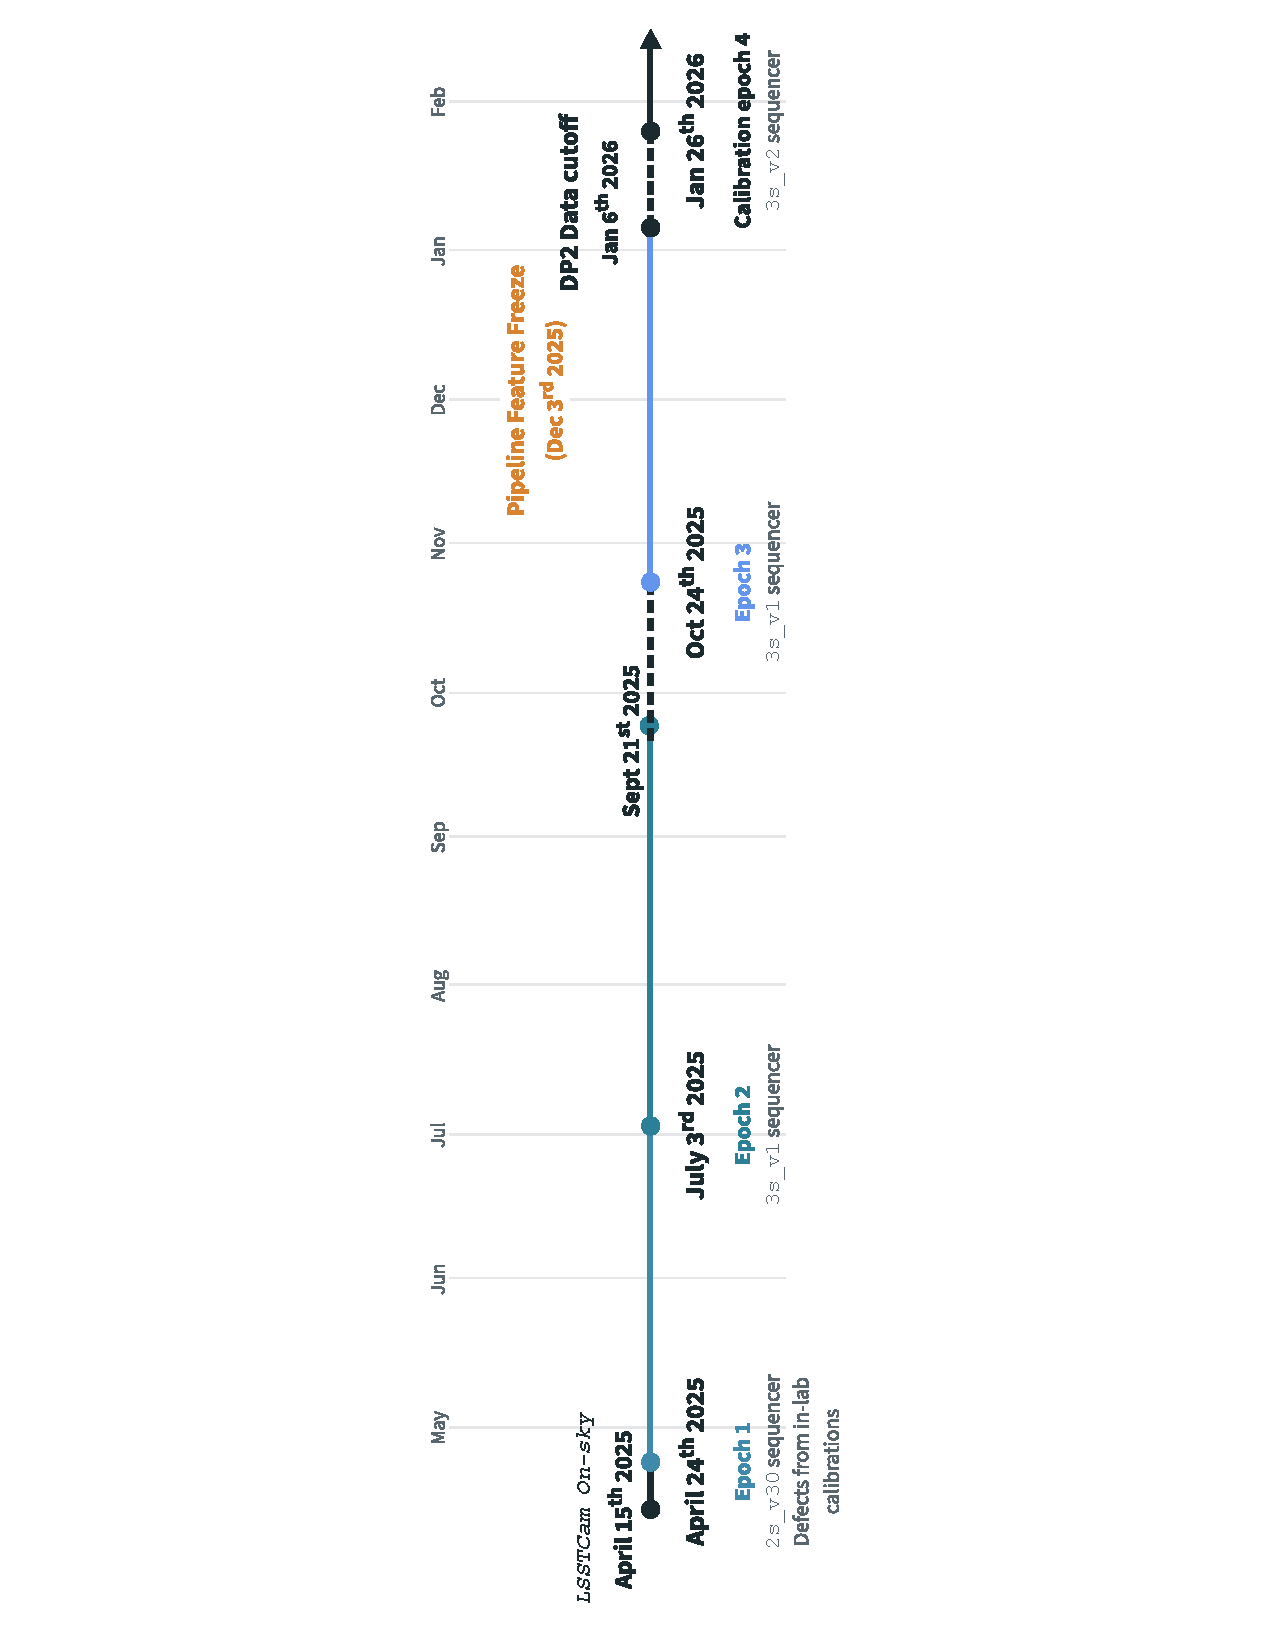
\includegraphics[trim=200bp 15bp 203bp 8bp, clip, angle=-90, width=\textwidth]{figures/calibration-epochs-timeline.pdf}
    \caption{Timeline of the observing periods and calibration epochs for LSSTCam during commissioning and pre-survey operations included in DP2. 
    The timeline begins on the day of LSSTCam first photon, soon after being mounted on the telescope. The first science data included in DP2 was taken on April 24th, 2025. Science data that was release as part of Data Preview 2 (DP2) is separated by calibration epochs, determined by changes to the CCD operating mode (sequencer) or power-cylces for maintenance. Colored segments denote the intervals covered by each calibration epoch: epoch~1 (from 2025 April 24)
    sequencer with calibrated defects derived from in-lab calibrations, epoch~2 (from 2025
    July 3, \texttt{3s\_v1}), and epoch~3 (from 2025 October 24, \texttt{3s\_v1}).
    Calibration epoch~4 (\texttt{3s\_v2}) follows the DP2 data cutoff on 2026
    January 6, 2026. The calibrations shown in this paper correspond to the most recent (\texttt{3s\_v2}) set of calibrations, despite the fact that no data from this period was released in DP2. 
    Dashed segments indicate intervals not covered by a calibration epoch, including an engineering/maintenence downtime between September 21-October 24, 2025. The code freeze for v30 of the LSST DM Science Pipelines software was December 3, 2025.}
    \label{fig:calibepoch}
\end{figure*}

